\documentclass[
	a4paper, % Paper size, specify a4paper (A4) or letterpaper (US letter)
	12pt, % Default font size, specify 10pt, 11pt or 12pt
]{class}

\addtolength{\textwidth}{1.75in}
\addtolength{\oddsidemargin}{-.850in}
\addtolength{\evensidemargin}{-.850in}

\usepackage{caption}
\usepackage{soul}
\usepackage{subcaption}

\addbibresource{bibliography.bib} % Bibliography file (located in the same folder as the template)

%----------------------------------------------------------------------------------------
%	REPORT INFORMATION
%----------------------------------------------------------------------------------------

\title{GPU Computing Project\\Parallel implementation of Dijkstra's Algorithm} % Report title

\author{Tricella Davide 08361A} % Author name(s), add additional authors like: '\& James \textsc{Smith}'

\date{\today} % Date of the report

%----------------------------------------------------------------------------------------

\begin{document}

\maketitle % Insert the title, author and date using the information specified above

\begin{center}
    \begin{tabular}{l r}
        Instructor: Professor \textsc{Grossi Giuliano}
    \end{tabular}
\end{center}

%----------------------------------------------------------------------------------------
%	ABSTRACT
%----------------------------------------------------------------------------------------

\begin{abstract}
    The purpose of this paper is to describe the implementation and benchmarking of various parallel implementations of Dijkstra's Algorithm to solve the all-pairs shortest path problem.
\end{abstract}

%----------------------------------------------------------------------------------------
%	TOC
%----------------------------------------------------------------------------------------

\tableofcontents
\newpage
%----------------------------------------------------------------------------------------
%	INTRODUCTION
%----------------------------------------------------------------------------------------

\section{Introduction}

The problem of shortest path in a graph consists in finding the path, from node A to node B,
which minimizes the sum of edges weights of which the path is composed.\\

\begin{center}
    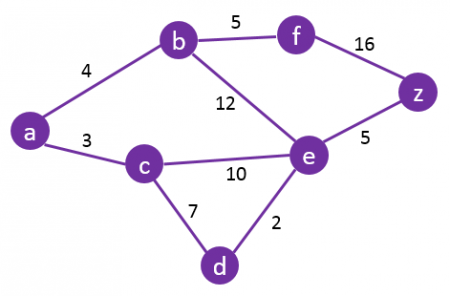
\includegraphics[width=10cm]{../images/graph.png}
    \captionof{figure}{Graph with edge weights}
\end{center}

In particular, the algorithm used for this document aim to solve the all-pairs shortest path problem,
which consists of finding the lenght of the shortest path for all the pairs of nodes.\\

The algorithm assumes that there are not negative weights and that the graph is undirected without isolated parts.\\

This problem is tackled in a lot of practical applications, like road networks path-finding, telecommunication routing and robot navigation.

\section{Dijkstra’s algorithm overview}
To solve the problem introduced before, there are several solutions which have been studied and improved troughout the years.
The option chosen for this task has been the Dijkstra’s algorithm, which has been implemented using the paper \cite{paper}
as a guidance.\\

This is a very well known algorithm, initially designed at the end of the 1950's, and used in a huge number of different applications.

The first version implemented was basically a parallel extension of the sequential algorithm,
then a more advanced approach has been taken for the improved version.

\newpage
\subsection{Sequential Version}
The basic algorithm solve the problem of shortest path between one Source Node and all the other nodes. The sequential version uses a for loop
to launch this version on every node of the graph, so at the end of the loop every node possesses the shortest path to every other node.\\

The main elements used during the computation are:\\
\begin{itemize}
    \item Graph Adiacency Matrix: which represents the graph indicating the weight of the edge which connects a node to another
    \item Vt Set: used as a stop condition and to check if a node has already a minimal path assigned
    \item l Array: which contains the minimal paths found for a certain node at a certain moment\\
\end{itemize}

We can divide the procedure into two main passages:\\
\begin{itemize}
    \item Initialization
    \item Main loop\\
\end{itemize}

During the first phase the Vt set is created containing only the Source Node, then the l Array is initialized, with the direct connections
from the Source Node to every other node, putting a symblic value of "infinity" where a direct connection is not available.\\

The the main loop begins, and continues until all the nodes are present in the Vt set. The Main cycle, is composed of two internal phases:\\
\begin{itemize}
    \item Local minimum search: between the elements of l not included in Vt we look for the minimum weight. Then we add the node selected to Vt.
    \item Update loop: the value of l corresponding to the node selected before gets updated with the minimum between the current value and the sum
    between the value selected during the minimum search and the weight present in the matrix. This part verifies if the value calculated by the search
    brings to a path actually shorter than the one stored.\\
\end{itemize}

When the Vt set is equal to the set of nodes of the graph, the Main loop terminates and the algorithm returns the l Array, 
where all the shortest paths are stored.\\

To solve the all pairs Shortest Paths problem we add an external loop that launch the algoritmh for every row of the original Adiacency Matrix,
and at the end returns a new matrix, composed of the various l arrays computed for every node.

\subsection{Basic parallel version}
The idea behind the initially implemented parallel version is simple:
to solve the problem we have to launch the algorithm |V| times, where V is the set of nodes of the graph.
Using only one block of the GPU, every thread executes the algorithm for one node of the graph, and at the end insert the results in the correct
row of the matrix in Global Memory.\\

The shared memory is not used because the variables needed for the computation are all locally present inside the thread, which is the main advantage of
this first technique, because there are not requirements of any kind on inter-process communications. Each thread works completely isolated from the others.\\

This implementation requires a thread per node of the graph, which still uses the various for loops present in the sequential version,
this fact make this implementation simple to program, with a decent speedup, provided the graph is big enough.\\
The main problem is that it is not taking full advantage of the Gpu capabilities, which is the weak spot that the second version tries to address. 

\subsection{Improved parallel version}
This version aim to exploit more the parallel execution of the GPU, using one Block per node of the graph, and one thread for every node to evaluate in the block.
To reach this objective it is necessary to use the shared memory to save the varius data used during the computation of a block.\\

This time the threads are not isolated and need to cooperate to compute the final array for the block result.
The inner for loop now implement a Parallel reduction procedure which compute the local minimum of a node.\\

There are some critical section of the code, like the stop condition check, that have been assigned exclusively to the first thread of the block,
using the thread syncronization directive, because these steps are not easy to parallelize, and the istruction executed by multiple threads could
cause concurrent acces which would slow down the evaluation.\\



\section{Implementation details}

\subsection{Sequential version}

\subsection{Basic parallel version}

\subsection{Improved parallel version}


\section{Benchmarking}

\subsection{Time usage}

\subsection{Memory usage}

\subsection{Profiling}

\newpage
\printbibliography % Output the bibliography

%----------------------------------------------------------------------------------------

\end{document}